\documentclass[9pt]{beamer}


\usepackage{adjustbox}
\usepackage{algorithm}
\usepackage{algpseudocode}
\usepackage{amsfonts}
\usepackage{amsmath}
\usepackage{amssymb}
\usepackage{amsthm}
\usepackage{array}
\usepackage{cite}
\usepackage{cuted}
\usepackage{environ}
\usepackage{graphicx}
\usepackage{grffile}
\usepackage{hyperref}
\usepackage{import}
\usepackage{lmodern}
\usepackage{mathtools}
\usepackage{microtype}
\usepackage{multirow}
\usepackage{pgfgantt}
\usepackage{pgfplots}
\usepackage{physics}
\usepackage{siunitx}
\usepackage{stfloats}
\usepackage{subcaption}
\usepackage{tikz}
\usepackage{url}
\usepackage{xcolor}
\usepackage[font=footnotesize,labelfont=bf]{caption}
\usepackage[RPvoltages]{circuitikz}
\usepackage[T1]{fontenc}
\usepackage[short]{optidef}


\interdisplaylinepenalty=2500
\pgfplotsset{compat=newest}
\usetikzlibrary{plotmarks}
\usetikzlibrary{arrows.meta}
\usepgfplotslibrary{patchplots}
\newtheorem{proposition}{Proposition}
\DeclareSIUnit{\belm}{Bm}
\DeclareSIUnit{\dBm}{\deci\belm}
\DeclareSIUnit{\beli}{Bi}
\DeclareSIUnit{\dBi}{\deci\beli}

\makeatletter
\newcommand{\forcealgorithm}{\let\@latex@error\@gobble}
\makeatother



\usepackage{circuitikz}
\ctikzset{american}
\usetikzlibrary{arrows,calc,matrix,patterns,positioning}

\makeatletter
\tikzset{
	block/.style={draw,rectangle,align=center},
    from/.style args={#1 to #2}{
        above right={0cm of #1},
        /utils/exec=\pgfpointdiff
            {\tikz@scan@one@point\pgfutil@firstofone(#1)\relax}
            {\tikz@scan@one@point\pgfutil@firstofone(#2)\relax},
        minimum width/.expanded=\the\pgf@x,
        minimum height/.expanded=\the\pgf@y
	}
}
\makeatother

\usepackage{siunitx}
\DeclareSIUnit{\belmilliwatt}{Bm}
\DeclareSIUnit{\dBm}{\deci\belmilliwatt}

\usepackage{blindtext}
\newcommand\blfootnote[1]{%
\begingroup
\renewcommand\thefootnote{}\footnote{#1}%
\addtocounter{footnote}{-1}%
\endgroup
}

\usepackage[acronym]{glossaries-extra}
\setabbreviationstyle[acronym]{long-short}
\newacronym{af}{AF}{Amplify-and-Forward}
\newacronym{ambc}{AmBC}{Ambient Backscatter Communication}
\newacronym{ap}{AP}{Access Point}
\newacronym{awgn}{AWGN}{Additive White Gaussian Noise}
\newacronym{bc}{BackCom}{Backscatter Communication}
\newacronym{bcd}{BCD}{Block Coordinate Descent}
\newacronym{bibo}{BIBO}{Binary-Input Binary-Output}
\newacronym{bpcu}{\si{bpcu}}{bit per channel use}
\newacronym{bpsphz}{\si{bps/Hz}}{bit per second per Hertz}
\newacronym{cscg}{CSCG}{Circularly Symmetric Complex Gaussian}
\newacronym{csi}{CSI}{Channel State Information}
\newacronym{df}{DF}{Decode-and-Forward}
\newacronym{dmc}{DMC}{Discrete Memoryless Channel}
\newacronym{dmtc}{DMTC}{Discrete Memoryless Thresholding Channel}
\newacronym{dtmac}{DTMAC}{Discrete memoryless Thresholding Multiple Access Channel}
\newacronym{dp}{DP}{Dynamic Programming}
\newacronym{gp}{GP}{Geometric Programming}
\newacronym{iid}{i.i.d.}{independent and identically distributed}
\newacronym{irs}{IRS}{Intelligent Reflecting Surface}
\newacronym{kkt}{KKT}{Karush–Kuhn–Tucker}
\newacronym{los}{LoS}{Line-of-Sight}
\newacronym{mac}{MAC}{Multiple Access Channel}
\newacronym{mc}{MC}{Multiplication Coding}
\newacronym{miso}{MISO}{Multiple-Input Single-Output}
\newacronym{mimo}{MIMO}{Multiple-Input Multiple-Output}
\newacronym{ml}{ML}{Maximum-Likelihood}
\newacronym{nfc}{NFC}{Near-Field Communication}
\newacronym{noma}{NOMA}{Non-Orthogonal Multiple Access}
\newacronym{ofdm}{OFDM}{Orthogonal Frequency-Division Multiplexing}
\newacronym{pdf}{PDF}{Probability Density Function}
\newacronym{psk}{PSK}{Phase Shift Keying}
\newacronym{pin}{PIN}{Positive Intrinsic-Negative}
\newacronym{qam}{QAM}{Quadrature Amplitude Modulation}
\newacronym{rf}{RF}{Radio Frequency}
\newacronym{rfid}{RFID}{Radio-Frequency Identification}
\newacronym{sc}{SC}{Superposition Coding}
\newacronym{sca}{SCA}{Successive Convex Approximation}
\newacronym{sic}{SIC}{Successive Interference Cancellation}
\newacronym{simo}{SIMO}{Single-Input Multiple-Output}
\newacronym{sinr}{SINR}{Signal-to-Interference-plus-Noise Ratio}
\newacronym{smawk}{SMAWK}{Shor-Moran-Aggarwal-Wilber-Klawe}
\newacronym{sr}{SR}{Symbiotic Radio}
\newacronym{tdma}{TDMA}{Time-Division Multiple Access}
\newacronym{tg}{TG}{tag}
\newacronym{tv}{TV}{television}
\newacronym{ue}{UE}{user}
\newacronym{wifi}{Wi-Fi}{Wi-Fi}


\usetheme{Warsaw}
\setbeamerfont{subsection in toc}{size=\footnotesize}

\AtBeginSection
{
    \begin{frame}
        \frametitle{Table of Contents}
        \tableofcontents[currentsection]
    \end{frame}
}

\title{Metascatter: \\Unifying Symbiotic Radio and Intelligent Reflecting Surface}
\author{Yang Zhao}
\institute{Department of Electrical and Electronic Engineering\\Imperial College London}
\date{Group Presentation, \today}

\begin{document}

	\frame{\titlepage}

	\begin{section}{Introduction and Review}
		\begin{subsection}{Literature Review}
			\begin{frame}{\glsentrylong{bc}}
				Backscatter allows wireless nodes to \alert{communicate} without active \glsentryshort{rf} chains on the tag.
				\begin{figure}[!t]
					\centering
					\subfloat[\glsentryshort{ambc} \cite{Zhao2017}]{
						\resizebox{0.35\columnwidth}{!}{
							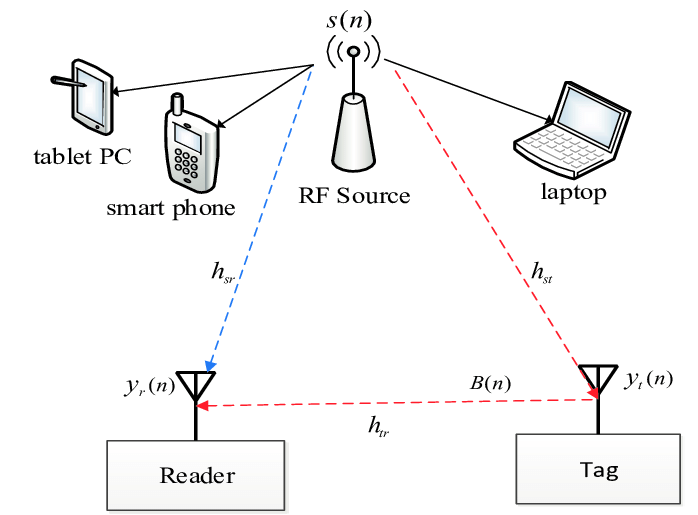
\includegraphics[width=0.5\textwidth]{assets/ambient_backscatter_system.png}
						}
						\label{fi:ambient_backscatter_system}
					}
					\subfloat[\glsentryshort{sr} \cite{Raza2022}]{
						\resizebox{0.55\columnwidth}{!}{
							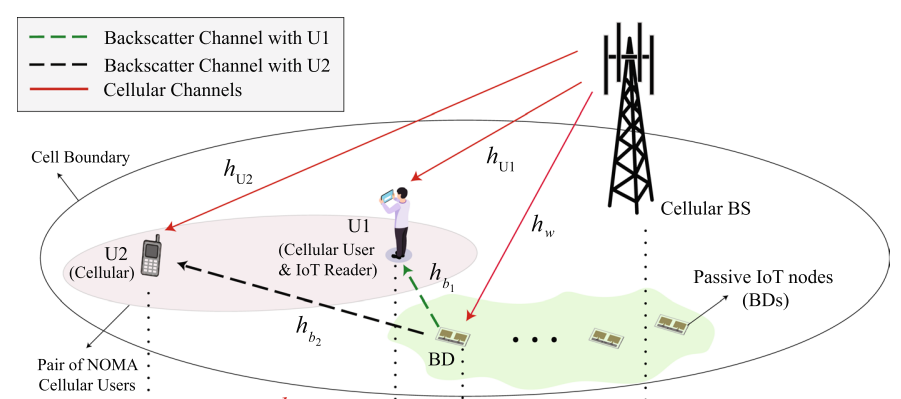
\includegraphics[width=0.9\textwidth]{assets/symbiotic_radio_system.png}
						}
						\label{fi:symbiotic_radio_system}
					}
				\end{figure}
				\begin{itemize}
					\item \textbf{\gls{ambc}} enables two battery-free devices to communicate over surrounding \glsentryshort{rf} signals.
					\item \textbf{\gls{sr}} also involves transmit and/or receive cooperation.
				\end{itemize}
			\end{frame}

			\begin{frame}{Passive Beamforming}
				Backscatter also enables real-time adaptive \alert{channel reconfiguration} using metamaterial.
				\begin{figure}[!t]
					\centering
					\subfloat[\glsentryshort{irs} architecture \cite{Wu2020}]{
						\resizebox{0.45\columnwidth}{!}{
							\includegraphics[width=0.9\linewidth]{assets/irs_architecture.eps}
						}
						\label{fi:irs_architecture}
					}
					\subfloat[\glsentryshort{irs} application \cite{Zhao2022}]{
						\resizebox{0.45\columnwidth}{!}{
							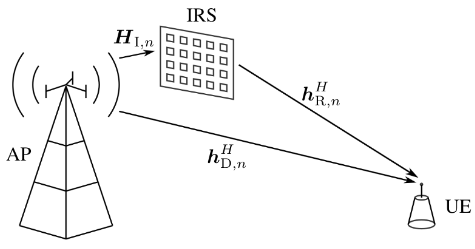
\includegraphics[width=0.9\linewidth]{assets/irs_application.png}
						}
						\label{fi:irs_application}
					}
				\end{figure}
				\begin{itemize}
					\item \textbf{\gls{irs}} controls the scattering properties of passive reflecting elements.
				\end{itemize}
			\end{frame}

			\begin{frame}{Properties of Backscatter Systems}
				\textbf{\gls{sr}}:
				\begin{itemize}
					\item Enable \alert{battery-less} transmission over \alert{legacy} systems
					\item Share \alert{spectrum, energy and infrastructures}
					\item Achieve flexible \alert{primary-backscatter tradeoff}
				\end{itemize}
				\vspace{1em}
				\textbf{\gls{irs}}:
				\begin{itemize}
					\item Enable \alert{real-time adaptive} channel reconfiguration for legacy systems
					\item Involve \alert{massive reflection} that benefits from array processing
					\item Achieve \alert{high passive beamforming gain}
				\end{itemize}
				\begin{table}
					\resizebox{\textwidth}{!}{
							\begin{tabular}{|l|l|l|l|l|}
								\hline
								Name                               & \glsentryshort{bc}  & \gls{irs}        & \gls{ambc}       & \gls{sr}                                 \\ \hline
								Coexisting systems (relationship)  & 1                   & 1                & 2 (competitive)  & 2 (collaborative)                        \\ \hline
								Transmitter role                   & Carrier emitter     & Source           & Carrier emitter  & Source and carrier emitter               \\ \hline
								Backscatter contribution           & Modulation          & Channel control  & Modulation       & Modulation and channel uncertainty       \\ \hline
								Spectrum and energy sharing        & No                  & No               & Yes              & Yes                                      \\ \hline
								Transceive cooperation             & --                  & --               & Neither          & Both                                     \\ \hline
								Operation range                    & Medium              & Long             & Short            & Short                                    \\ \hline
								Backscatter detection              & Coherent            & --               & Non-coherent     & Coherent (typically \glsentryshort{sic}) \\ \hline
							\end{tabular}
					}
				\end{table}
			\end{frame}
		\end{subsection}

		\begin{subsection}{Backscatter Principles}
			\begin{frame}{Tag Structure}
				Passive tags harvest energy from and modulate information over incident signal.
				\begin{figure}[!t]
					\centering
					\subfloat[Passive tag structure]{
						\resizebox{0.5\columnwidth}{!}{
							\begin{circuitikz}[transform shape]
								\coordinate (O) at (0,0);
								\node[block,from={O to $(O) + (6.375,3.25)$}](T){};
								\draw (0,1.75)
									to[short] ++(-0.875,0)
									to[short] ++(0,0.5) node[bareantenna](A){Bx};
								\draw (0,1.75)
									to[short,-*] ++(0.25,0) coordinate(J);
								\draw (J)
									to[short] ++(0,1)
									to[short] ++(0.5,0) coordinate(J1);
								\node[block,from={$(J1) + (0,-0.25)$ to $(J1) + (2.5,0.25)$}](R){Rectifier};
								\draw (J)
									to[short] ++(0.5,0) coordinate(J2);
								\node[block,from={$(J2) + (0,-0.25)$ to $(J2) + (2.5,0.25)$}](D){Demodulator};
								\draw (J)
									to[short] ++(0,-1)
									to[short] ++(0.5,0) coordinate(J3)
									to [vR,mirror,invert,/tikz/circuitikz/bipoles/length=1cm] ++(1.75,0) node[ground,rotate=90]{};
								\node[block,from={$(J3) + (0,-0.25)$ to $(J3) + (2.5,0.25)$},draw=none](M){};
								\draw ($(J3) + (0,-0.25)$) rectangle ($(J3) + (2.5,0.25)$);
								\draw ($(J3) + (1.25,-0.5)$) node[]{Modulator};
								\draw[-{Latex[length=2mm]}] (R.east) -- ++(0.75,0);
								\draw[-{Latex[length=2mm]}] (D.east) -- ++(0.75,0);
								\draw[{Latex[length=2mm]}-] (M.east) -- ++(0.75,0);
								\node[block,from={$(R.east) + (0.75,-0.25)$ to $(R.east) + (2.875,0.25)$}](P){Power buffer};
								\node[block,from={$(M.east) + (0.75,-0.25)$ to $(D.east) + (2.875,0.25)$}](S){Digital\\section};
								\draw[dashed,-{Latex[length=2mm]}] (P.south) to (S.north);
								\coordinate (F1) at ($(P.south)!0.5!(S.north)$);
								\coordinate (F2) at ($(D.east)!0.5!(S.west)$);
								\coordinate (F3) at ($(D.south)!0.5!(M.north)$);
								\draw[dashed] (F1) to (F1-|D.north);
								\draw[dashed,-{Latex[length=2mm]}] (F1-|D.north) to (D.north);
								\draw[dashed] (F1-|F2) to (F2|-F3) to (M|-F3);
								\draw[dashed,-{Latex[length=2mm]}] (M|-F3) to (M.north);
							\end{circuitikz}
						}
						\label{fi:passive_tag_structure}
					}
					\subfloat[\glsentryshort{rfid} tag with energy harvesting module \cite{Molina-Farrugia2017}]{
						\resizebox{0.45\columnwidth}{!}{
							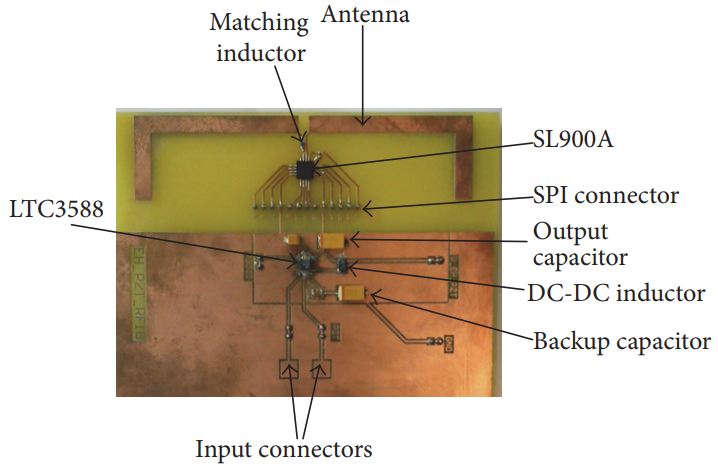
\includegraphics[width=0.9\linewidth]{assets/passive_tag_prototype.png}
						}
						\label{fi:passive_tag_prototype}
					}
				\end{figure}
			\end{frame}

			\begin{frame}{Backscatter Model}
				\begin{figure}[!t]
					\centering
					\subfloat[Tag equivalent circuit]{
						\resizebox{0.65\columnwidth}{!}{
							\begin{circuitikz}[transform shape]
								\draw (0,0) coordinate(O)
									to [sV,l=$V_0$] ++(0,1.5)
									to [L,l=$X_{\mathrm{A}}$] ++(0,1.5)
									to [R=$R_{\mathrm{R}}$,-*] ++(3,0) coordinate(AM)
									to [sI,l_=$I_0$,-*] ++(0,-3)
									to [short] (O);
								\draw (AM)
									to [short] ++(0.5,0)
									to [L,l=$X_{\mathrm{M}}$,-*] ++(3,0) coordinate(M)
									to [R=$R_{\mathrm{M},2}$] ++(3,0) coordinate(MH);
								\draw (M)
									to [R=$R_{\mathrm{M},1}$,-*] ++(0,-3);
								\draw (MH)
									to [D,-*] ++(1.5,0) coordinate(H)
									to [C=$X_{\mathrm{H}}$,-*] ++(0,-3);
								\draw (H)
									to [short] ++(1.5,0)
									to [R=$R_{\mathrm{C}}$] ++(0,-3)
									to [short] (O);

								\draw [blue,dashed] (-1.25,-0.5) rectangle (3.5,3.75);
								\draw [yellow,dashed] (4,-0.5) rectangle (9,3.75);
								\draw [red,dashed] (9.5,-0.5) rectangle (13.5,3.75);

								\draw [blue] (1.125,4) node[]{Antenna};
								\draw [yellow] (6.5,4) node[]{Modulator};
								\draw [red] (11.5,4) node[]{Harvester + Chip};

								\draw (3.375,2.675) to [short] (3.375,3.175) to [short] (3.25,3.175) to [short,i_=$Z_{\mathrm{A}}$] (3.125,3.175);
								\draw (4.125,-0.125) to [short] (4.125,0.375) to [short] (4.25,0.375) to [short,i=$Z_m$] (4.375,0.375);
								\draw (9.625,-0.125) to [short] (9.625,0.375) to [short] (9.75,0.375) to [short,i=$Z_{\mathrm{H}}$] (9.875,0.375);
							\end{circuitikz}
						}
						\label{ci:tag_equivalent_circuit}
					}
					\subfloat[Backscatter model]{
						\resizebox{0.3\columnwidth}{!}{
							\begin{circuitikz}[transform shape]
								\draw (0,0) node[bareantenna](bareantenna){};
								\draw (bareantenna.west) ++(-1.5,0) node[waves](WI){};
								\draw (WI.north east) ++(0.25,0) node[font=\Large]{$\vec{E}_{\mathrm{I}}$};
								\draw (WI.south east) ++(0.25,0) node[font=\Large]{$\vec{H}_{\mathrm{I}}$};
								\draw (bareantenna.east) ++(0.875,0) node[waves](WR){};
								\draw (WR.north east) ++(0.35,0) node[font=\Large]{$\vec{E}_m$};
								\draw (WR.south east) ++(0.35,0) node[font=\Large]{$\vec{H}_m$};
								\draw (bareantenna)
									to [R=$Z_{\mathrm{A}}$,font=\Large,/tikz/circuitikz/bipoles/length=1cm] ++(0,-1.5) node[rotary switch=4 in 90 wiper 30,anchor=ext center,rotate=270](SW){};
								\draw (SW.cout 2) node[below=0.1cm,font=\Large]{$m$}
									to [R=$Z_m$,font=\Large,/tikz/circuitikz/bipoles/length=1cm] ++(2,0) node[ground]{};
							\end{circuitikz}
						}
						\label{fi:backscatter_model}
					}
				\end{figure}
				The complex reflection coefficient depends on the antenna-load impedance matching
				\begin{equation}
					\Gamma_m \triangleq \frac{Z_m - Z_{\mathrm{A}}^*}{Z_m + Z_{\mathrm{A}}},
					\label{eq:reflection_coefficient}
				\end{equation}
				which controls the \alert{amplitude} and \alert{phase} of the backscatter signal.
			\end{frame}

			\begin{frame}{Reflection Coefficient}
				\textbf{\gls{sr}} \alert{varies} the reflection coefficient for backscatter modulation
				\begin{equation}
					\Gamma_m = \alpha \frac{c_m}{\max_{m'} \lvert c_{m'} \rvert}.
					\label{eq:backscatter_modulation}
				\end{equation}
				\textbf{\gls{irs}} \alert{chooses the best} reflection coefficient for passive beamforming
				\begin{equation}
					\Gamma_m = \beta_m \exp(j \theta_m).
					\label{eq:passive_beamforming}
				\end{equation}

				\begin{block}{Question}
					For a given reflector, is it possible to merge \gls{sr} and \gls{irs} by proper reflection coefficient selection?
				\end{block}
			\end{frame}
		\end{subsection}
	\end{section}

	\begin{section}{Metascatter}
		\begin{subsection}{System Model}
			\begin{frame}{Metascatter tags}
				\textbf{Metascatter} adapts the \alert{probability distribution} of tag states to unify backscatter modulation and passive beamforming.
				\begin{columns}
					\begin{column}{0.625\columnwidth}
						If all \glsentryshort{csi} can be estimated,
						\begin{itemize}
							\item \gls{irs} chooses the best state with probability \num{1}
							\item \gls{sr} assumes all input letters are equiprobable
							\item Metascatter enables flexible input design
						\end{itemize}
					\end{column}
					\begin{column}{0.375\columnwidth}
						\begin{figure}[!t]
							\centering
							\resizebox{\columnwidth}{!}{
								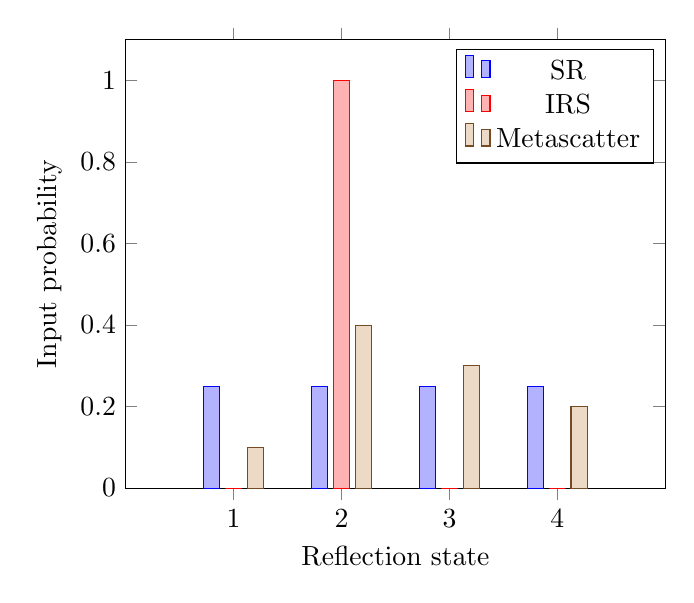
\begin{tikzpicture}
									\begin{axis}[
											ybar,
											bar width = 0.15,
											xmin = 0,
											xmax = 4,
											xtick = data,
											ymin = 0,
											ymax = 1,
											xlabel={Reflection state},
											ylabel={Input probability},
											enlarge x limits = {value = 0.25, upper},
											enlarge y limits = {value = 0.1, upper}
										]
										\addplot coordinates {(1,0.25) (2,0.25) (3,0.25) (4,0.25)};
										\addplot coordinates {(1,0) (2,1) (3,0) (4,0)};
										\addplot coordinates {(1,0.1) (2,0.4) (3,0.3) (4,0.2)};
										\legend {SR, IRS, Metascatter};
									\end{axis}
								\end{tikzpicture}
							}
							\caption{Tag probability distribution.}
						\end{figure}
					\end{column}
				\end{columns}
			\end{frame}

			\begin{frame}{Metascatter System}
				Assume the backscatter pattern of all tags change per $N \gg 1$ primary symbols.

				\vspace{1em}
				\begin{figure}[!t]
					\centering
					\def\svgwidth{0.7\columnwidth}
					\import{assets/}{metascatter_system.eps_tex}
					\caption{The proposed Metascatter system.}
					\label{fi:metascatter_system}
				\end{figure}
				The received signal is
				\begin{equation}
					y[n] = \underbrace{\left(\boldsymbol{h}_{\mathrm{D}}^H + \sum_{k \in \mathcal{K}} \sqrt{\alpha_k} \boldsymbol{h}_{\mathrm{C},k}^H \alert{x_k}\right)}_{\boldsymbol{h}_{\mathrm{E}}^H(x_{\mathcal{K}})} \boldsymbol{w} \alert{s[n]} + w[n].
					\label{eq:received_signal}
				\end{equation}
				% Recycle the ambient \glsentryshort{rf} signal in an efficient manner.
			\end{frame}

			\begin{frame}{Metascatter Decoding}
				We first \alert{jointly} and \alert{non-coherently} decode all backscatter symbols. The accumulated energy $z$ over $N$ primary symbol duration follows Erlang distribution
				\begin{equation}
					f(z \mid \mathcal{H}_{m_{\mathcal{K}}}) = \frac{z^{N-1} e^{-z/\sigma_{m_{\mathcal{K}}}^2}}{\sigma_{m_{\mathcal{K}}}^{2N} (N-1)!}
					\label{eq:energy_distribution}
				\end{equation}

				\vspace{1em}
				The backscatter decoding involves \alert{decision region threshold} design over $z$.
				\begin{figure}
					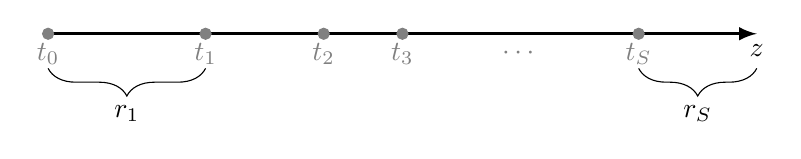
\begin{tikzpicture}
						\draw[very thick,-latex] (0,0) -- (9,0) node[below]{$z$};
						\filldraw [gray] (0,0) circle (2pt) node[below]{$t_0$};
						\filldraw [gray] (2,0) circle (2pt) node[below]{$t_1$};
						\filldraw [gray] (3.5,0) circle (2pt) node[below]{$t_2$};
						\filldraw [gray] (4.5,0) circle (2pt) node[below]{$t_3$};
						\filldraw [gray] (7.5,0) circle (2pt) node[below]{$t_S$};
						\node[gray] at (6,-0.25) {$\cdots$};
						\draw[decorate,decoration={brace,mirror,amplitude=10},xshift=0,yshift=-12.5] (0,0) -- (2,0) node[below,midway,yshift=-10]{$r_1$};
						\draw[decorate,decoration={brace,mirror,amplitude=10},xshift=0,yshift=-12.5] (7.5,0) -- (9,0) node[below,midway,yshift=-10]{$r_S$};
					\end{tikzpicture}
					\caption{Decision region for each letter may contain disjoint partitions.}
				\end{figure}
			\end{frame}

			\begin{frame}{Metascatter Decoding}
				The transition probability from channel input $x_{m_{\mathcal{K}}}$ to output $\hat{x}_{m_{\mathcal{K}}'}$ is
				\begin{equation}
					P(\hat{x}_{m_{\mathcal{K}}'} \mid x_{m_{\mathcal{K}}}) = \int_{\mathcal{R}_{m_{\mathcal{K}}'}} f(z \mid \mathcal{H}_{m_{\mathcal{K}}}) \dd z.
					\label{eq:dtmac}
				\end{equation}

				\vspace{1em}
				Once successfully recovered, the backscatter symbols are \alert{modeled within} equivalent channel for primary decoding.
			\end{frame}

			\begin{frame}{Achievable Rates}
				Denote the input probability of tag $k$ at state $m_k$ as $P_k(x_{m_k})$, and the probability of input combination $x_{m_{\mathcal{K}}}$ as $P_{\mathcal{K}}(x_{m_{\mathcal{K}}}) = \prod_{k \in \mathcal{K}} P_k(x_{m_k})$ (independent encoding).

				\vspace{1em}
				The backscatter achievable rate is
				\begin{equation}
					I_{\mathrm{B}}(x_{\mathcal{K}};\hat{x}_{\mathcal{K}}) = \sum_{m_{\mathcal{K}}} P_{\mathcal{K}}(x_{m_{\mathcal{K}}}) \sum_{m_{\mathcal{K}}'} P(\hat{x}_{m_{\mathcal{K}}'} \mid x_{m_{\mathcal{K}}}) \log \frac{P(\hat{x}_{m_{\mathcal{K}}'} \mid x_{m_{\mathcal{K}}})}{P(\hat{x}_{m_{\mathcal{K}}'})}.
					\label{eq:backscatter_mutual_information}
				\end{equation}
				The primary (ergodic) rate is
				\begin{equation}
					I_{\mathrm{P}}(x_{\mathcal{K}};\boldsymbol{y}) = \sum_{m_{\mathcal{K}}} P_{\mathcal{K}}(x_{m_{\mathcal{K}}}) N \log_2 \left(1 + \frac{\lvert \boldsymbol{h}_{\mathrm{E}}^H(x_{m_{\mathcal{K}}}) \boldsymbol{w} \rvert^2}{\sigma_w^2}\right).
					\label{eq:primary_mutual_information}
				\end{equation}
				The achievable rates depend on \alert{tag input distribution, energy decision threshold, and transmit precoder design.}
			\end{frame}
		\end{subsection}

		\begin{subsection}{Input, Threshold and Precoder Optimization}
			\begin{frame}{Optimization Problem}
				We aim to characterize the primary-(sum-)backscatter rate region.
				\begin{maxi!}
					{\scriptstyle{\{\boldsymbol{p}_k\},\boldsymbol{t},\boldsymbol{w}}}{I(x_{\mathcal{K}};\hat{x}_{\mathcal{K}},\boldsymbol{y}) \triangleq \rho I_{\mathrm{P}}(x_{\mathcal{K}};\boldsymbol{y}) + (1 - \rho) I_{\mathrm{B}}(x_{\mathcal{K}};\hat{x}_{\mathcal{K}})}{\label{op:weighted_sum_rate}}{\label{ob:weighted_sum_rate}}
					\addConstraint{\sum \nolimits_{m_k} P_k(x_{m_k})}{=1,}{\quad \forall k \in \mathcal{K}}{\label{co:sum_probability}}
					\addConstraint{P_k(x_{m_k})}{\ge 0,}{\quad \forall k \in \mathcal{K}, \ \forall m_k \in \mathcal{M}}{\label{co:nonnegative_probability}}
					\addConstraint{\lVert \boldsymbol{w} \rVert^2}{\le P.}{\label{co:transmit_power}}
				\end{maxi!}
				Since problem \eqref{op:weighted_sum_rate} is not jointly convex, we propose a \glsentryshort{bcd} algorithm that iteratively updates $\{\boldsymbol{p}_k\}$, $\boldsymbol{t}$ and $\boldsymbol{w}$ until convergence.
			\end{frame}

			\begin{frame}{Input Probability Distribution}
				For a given threshold and precoder, the input distribution design is non-convex when $K > 1$.
				\begin{itemize}
					\item \glsentryshort{gp} needs to approximate $\prod_{k \in \mathcal{K}} P_k(x_{m_k}) \log \prod_{k \in \mathcal{K}} P_k(x_{m_k})$ with high complexity
					\item \glsentryshort{sca} and \glsentryshort{kkt} solutions are trapped at saddle points
				\end{itemize}
				\begin{block}{\glsentryshort{kkt} Solution}
					The \glsentryshort{kkt} solution is given by the converging point of the sequence
					\begin{equation}
						P_k^{(r+1)}(x_{m_k}) = \frac{P_k^{(r)}(x_{m_k}) \exp \left( \frac{\rho}{1 - \rho} I_k^{(r)}(x_{m_k};\hat{x}_{\mathcal{K}},\boldsymbol{y}) \right)}{\sum_{m_k'} P_k^{(r)}(x_{m_k'}) \exp \left( \frac{\rho}{1 - \rho} I_k^{(r)}(x_{m_k'};\hat{x}_{\mathcal{K}},\boldsymbol{y}) \right)},
						\label{eq:input_kkt_solution}
					\end{equation}
					where $r$ is the iteration index and $\boldsymbol{p}_k^{(0)} > \boldsymbol{0}$, $\forall k \in \mathcal{K}$.
				\end{block}
			\end{frame}

			\begin{frame}{Transmit Precoder}
				The optimal precoder design is highly non-convex that involves integration, entropy term, and variable on exponential. We may propose a suboptimal precoder based on linear combination of equivalent and cascaded channels, or consider single transmit antenna instead.
			\end{frame}

			\begin{frame}{Decision Threshold}
				Once the input distribution is determined, \eqref{eq:dtmac} becomes a point-to-point channel since total backscatter rate is considered.

				\vspace{1em}
				\begin{block}{Minimum Number of Thresholds}
					The minimum number of distinct thresholds for problem \eqref{op:weighted_sum_rate} is $L+1$ if there are $L$ input combinations with non-zero probability.
				\end{block}
				\vspace{1em}
			\end{frame}
		\end{subsection}
	\end{section}

	\begin{section}{\glsentryshort{dp}-Based Threshold Design}
		\begin{frame}{System Model}
			\cite{He2021} aims to obtain the optimal $M$-level quantizer for \glsentryshort{dmc} with $q$ inputs and $N$ outputs.
			\begin{figure}
				\resizebox{0.45\columnwidth}{!}{
					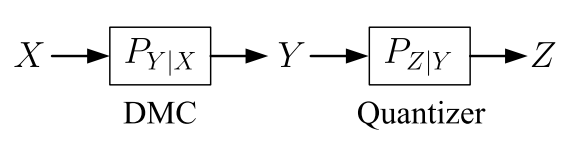
\includegraphics[width=0.5\linewidth]{assets/dmtc.png}
				}
				\caption{Quantization of \glsentryshort{dmc} \cite{He2021}}
			\end{figure}
			Essentially, the continuous output is discretized into $N$ fine-grained bins.
		\end{frame}

		\begin{frame}{Quantization cost}
			Preliminary:
			\begin{itemize}
				\item There exists a deterministic quantizer that is optimal
				\item The optimal quantizer is convex w.r.t. backward channel $P(X|Y)$
			\end{itemize}

			\vspace{1em}
			The cost of quantizing $\{y_l,\ldots,y_r\}$ into one level is
			\begin{equation}
				w(l,r) = \sum_{j'=l}^r P_Y(y_{j'}) \phi \left(\frac{\sum_{j=l}^r P_{X,Y}(\cdot,y_j)}{\sum_{j''=l}^r P_Y(y_{j''})}\right).
			\end{equation}
		\end{frame}

		\begin{frame}{\glsentrylong{dp}}
			The aim is to minimize the sum cost of allocating $N$ bins to $M$ letters.

			\vspace{1em}
			It can be simplified by considering subproblem, to quantize $n < N$ bins into $m < M$ letters.

			\vspace{1em}
			The core idea is to bridge the optimal cost function of subproblems when $m$ increases, and shrink the search range based on existing results.
		\end{frame}

		\begin{frame}{\glsentryshort{smawk}}
			\glsentryshort{smawk} algorithm \cite{Aggarwal1986} is designed to find the minimum value in each row of a monotone matrix. It can accelerate \glsentryshort{dp} if the problem satisfies some nice properties.

			\vspace{1em}
			Two reductions are applied alternately and recursively:
			\begin{itemize}
				\item Interpolate (when more rows or equal): eliminate odd rows
				\item Reduce (when more columns): find the first index in a row when next element is bigger, then go to next row and start from that index; eliminate all unindexed columns
			\end{itemize}
		\end{frame}

		\begin{frame}{Result of \cite{He2021}}
			\begin{figure}[!t]
				\centering
				\resizebox{0.6\columnwidth}{!}{
					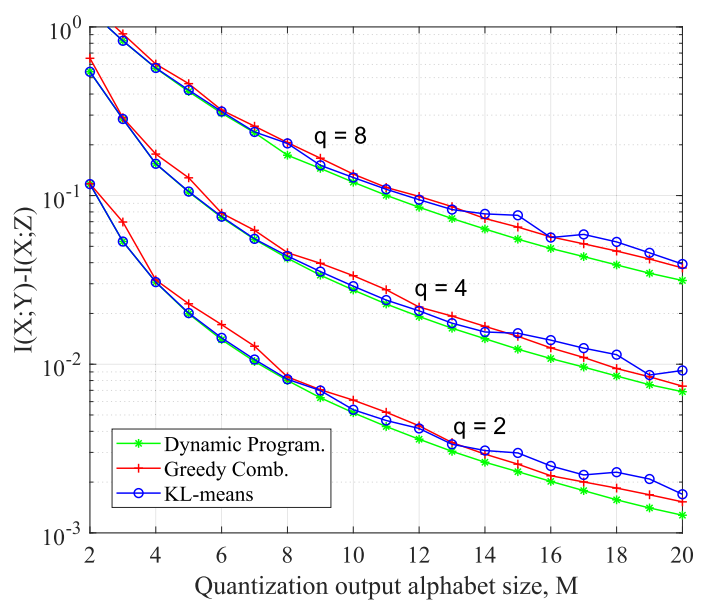
\includegraphics{assets/dp_result.png}
				}
			\end{figure}
			The \glsentryshort{dp} design achieves global optimality with complexity $\mathcal{O}(q(N-M)M)$.
		\end{frame}
	\end{section}

	\begin{section}{Preliminary Results}
		\begin{frame}{Parameters}
			\begin{table}[t!]
				\centering
				\caption{Parameters in simulation}
				\begin{tabular}{ll}
					Transmit antenna $Q$          & 1     \\
					Tags $K$                      & 2     \\
					States $M$                    & 2     \\
					Reflect ratio $\alpha$        & 0.5   \\
					Duration ratio $N$            & 10    \\
					Noise power $\sigma_w^2$      & 1     \\
					Discretization bins           & 256
				\end{tabular}
				\label{ta:parameters}
			\end{table}
		\end{frame}

		\begin{frame}{Schemes}
			Input probability distribution schemes:
			\begin{itemize}
				\item Cooperation: assume full transmit cooperation (joint encoding) at all tags
				\item Exhaustion: evaluate and compare all possible input distributions
				\item \glsentryshort{kkt}: solution by \eqref{eq:input_kkt_solution}
				\item Marginalization: marginalize the joint input array by Cooperation
			\end{itemize}

			Decision threshold schemes:
			\begin{itemize}
				\item \glsentryshort{smawk}: aforementioned \glsentryshort{dp}-based searching method \cite{He2021}
				\item Bisection: sequentially optimizes each threshold by bisection \cite{Nguyen2020a}
				\item \glsentryshort{ml}: requires no input distribution knowledge \cite{Qian2019}
			\end{itemize}
		\end{frame}

		\begin{frame}{Results}
			\begin{figure}[!t]
				\centering
				\resizebox{0.8\columnwidth}{!}{
					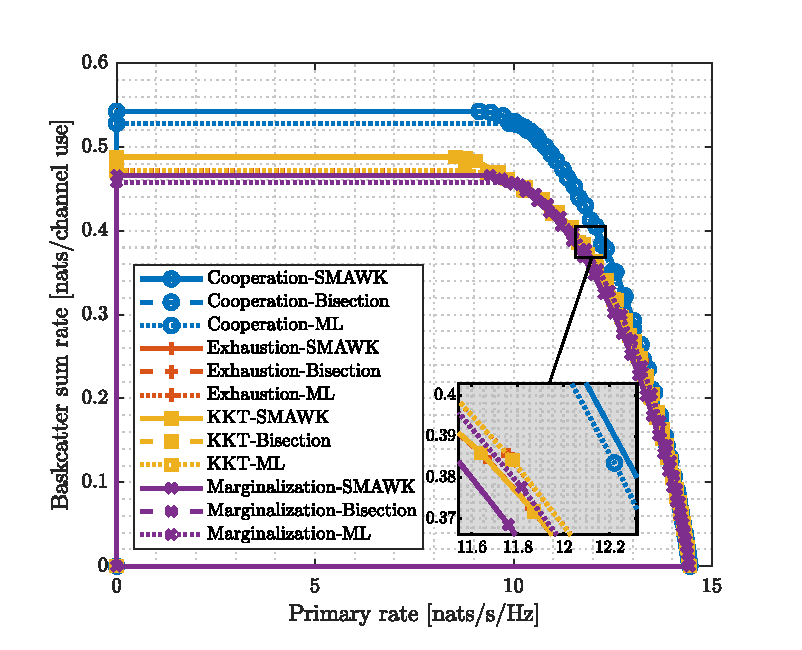
\includegraphics{assets/rate_region_1.eps}
				}
				\caption{Achievable rate regions by input-threshold design: Case I.}
				\label{fi:rate_region_1}
			\end{figure}
		\end{frame}

		\begin{frame}{Results}
			\begin{figure}[!t]
				\centering
				\resizebox{0.8\columnwidth}{!}{
					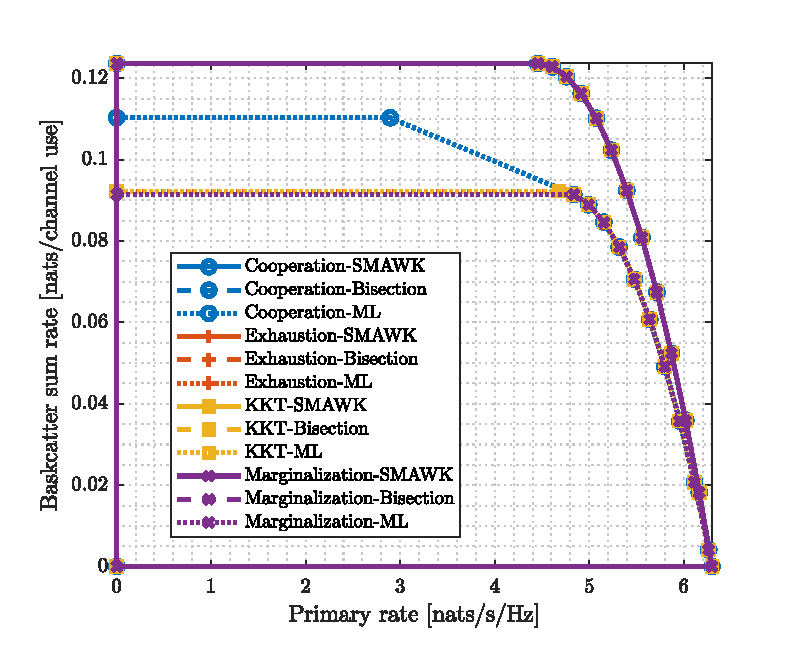
\includegraphics{assets/rate_region_2.eps}
				}
				\caption{Achievable rate regions by input-threshold design: Case II.}
				\label{fi:rate_region_2}
			\end{figure}
		\end{frame}
	\end{section}

	\bibliographystyle{IEEEtran}
	\bibliography{IEEEabrv,library.bib}
\end{document}
